%\chapter{Disk Arrangement}
\chapter{Realizability Problems for Weighted Trees}\label{chp:disk}
\section{Properties for Weighted Trees and Polygonal Linkages}
In order to perform our analysis for weighted trees and polygonal linkages, we'll want to use a suitable metric.  
The usual Euclidian distance will not suffice for this analysis and so we turn to the Hausdorff distance.
\paragraph{Hausdorff Distance}  Let $A$ and $B$ be sets in the plane. The \textit{directed Hausdorff distance} is 
\begin{equation}\label{eqn:ContactGraphV3-1}
d\lr{A,B} = \sup_{a \in A} \inf_{b \in B} \left\vert\left\vert a-b \right\vert \right\vert
\end{equation}
$h\lr{A,B}$ finds the furthest point $a \in A$ from any point in $B$.  \textit{Hausdorff distance} is
\begin{equation}\label{eqn:ContactGraphV3-2}
D\lr{A,B} = \max \left\lbrace d\lr{A,B}, d\lr{B,A} \right\rbrace
\end{equation}
\begin{figure}[!htbp]
\begin{center}
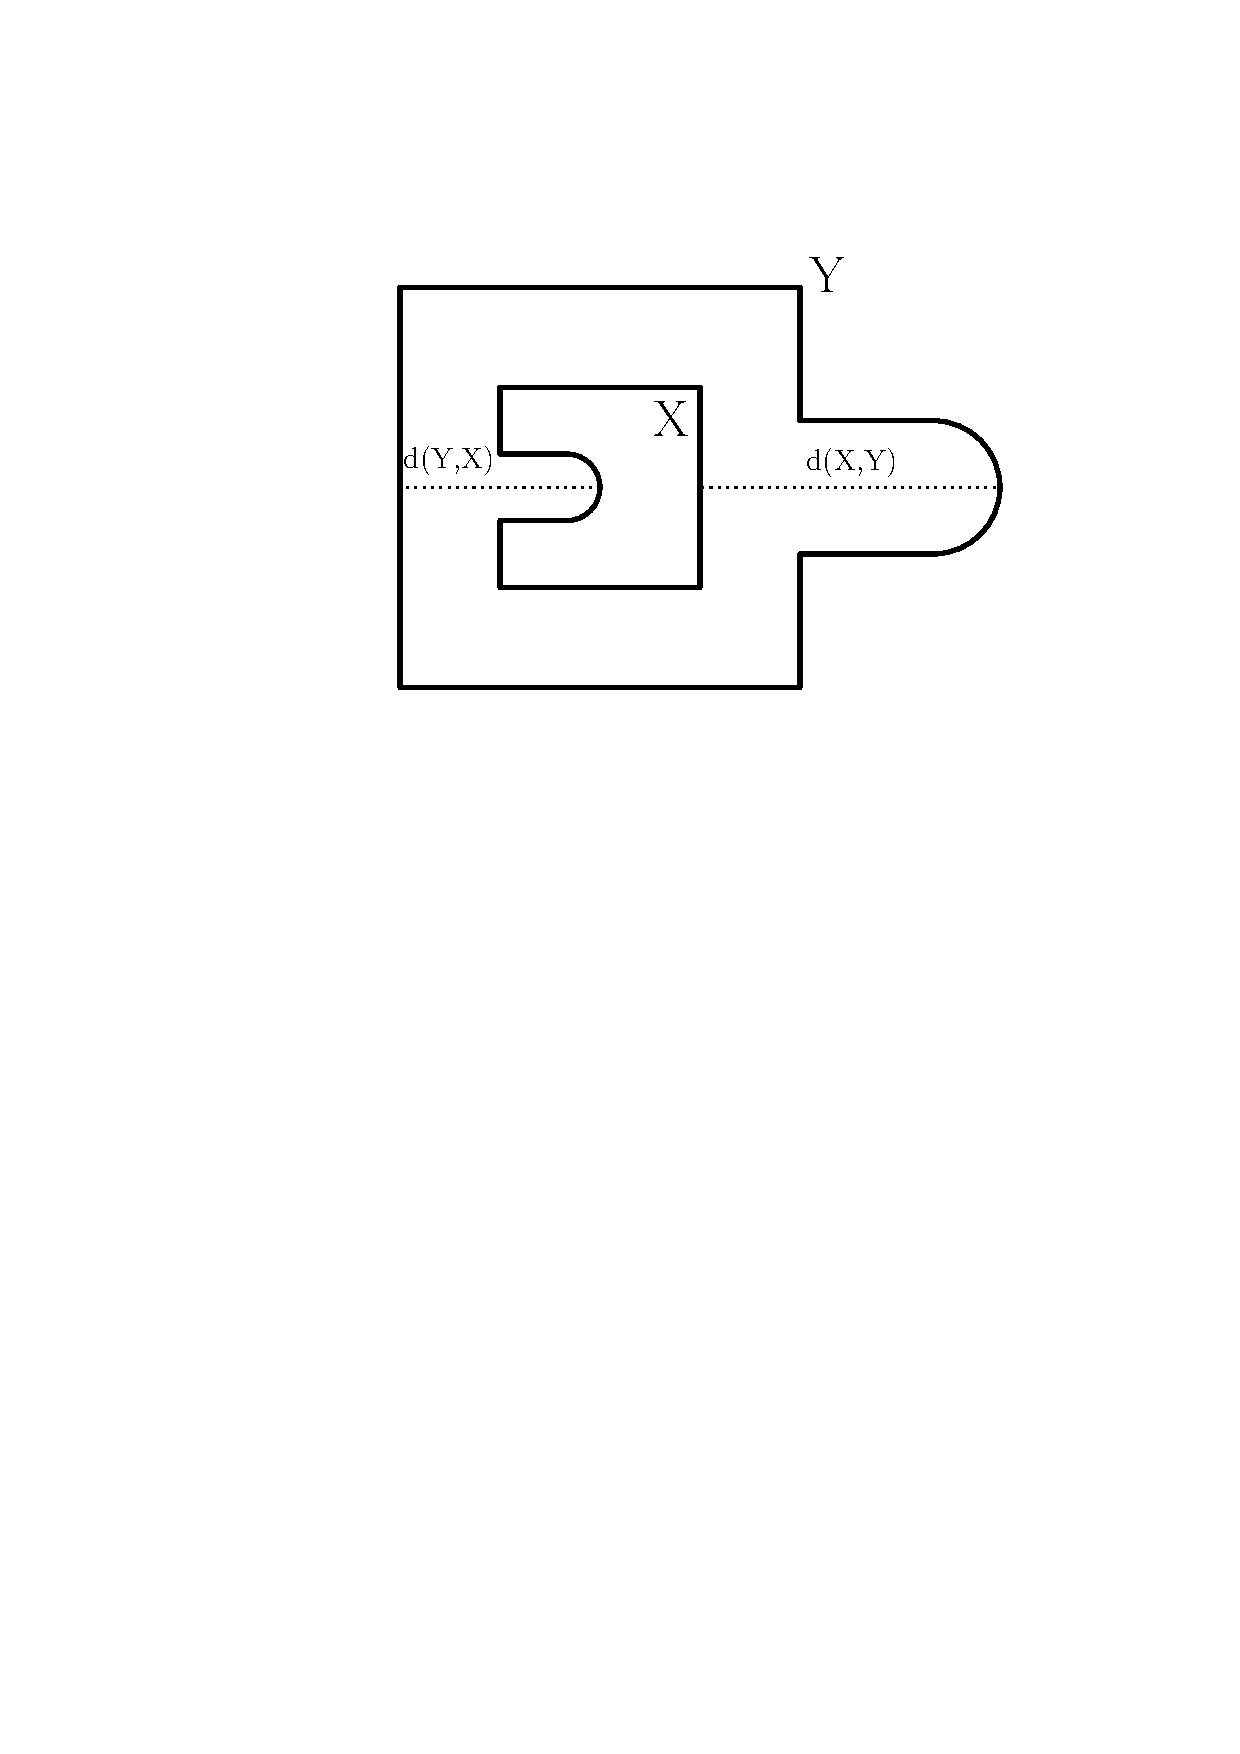
\includegraphics[scale=.5]{graphics/HausdorffDistanceExample1.pdf}
\caption{An illustrative example of $d(X,Y)$ and $d(Y,X)$ where $X$ is the inner curve, and $Y$ is the outer curve.}\label{fig:HausdorffDistanceExample1.pdf}
\end{center}
\end{figure}
\paragraph{$\epsilon$-approximation}
% Modeling the logic engine with polygonal linkages requires reflected copies of the
% rectangles. For an oriented realization, we use a different technique in Section 3. The
% above proof can be adapted to the realization of contact trees of disks by approximating
% rectangles with disk arrangements. In this context, we say that a weighted graph G is a
% ε-approximation of a polygon P if G is realizable as a contact graph of disks of given
% radii, and in every such realization, the Hausdorff distance between the union of disks
% and a congruent copy of P is at most ε. A weighted graph G is a stable ε-approximation
% if, in addition, for every two such realizations of G, the distance between the centers of
% the corresponding disks is at most ε after a suitable rigid transformation.
The weighted graph, $G$, is an \textit{$\epsilon$-approximation} of a polygon $P$ if the Hausdorff distance between every realization such realization of $G$ as a contact graph of disks and a congruent copy of $P$ is at most epsilon.  
A weighted graph $G$ is said to be a \textit{$\BigOh{f(x)}$-approximation} of a polygon P if there is a positive constant $M$ such that for all sufficiently large values of $x$ the Hausdorff distance between every realization such realization of $G$ as a contact graph of disks and a congruent copy of $P$ is at $M \cdot \vert f(x)\vert$. 
A weighted graph $G$ is said to be a \textit{stable} if it has the property that for every two such realizations of $G$, the distance between the centers of the corresponding disks is at most $\epsilon$ after a suitable rigid transformation.